\section{MKA Overview}
\label{sec:background}

\subsection{IEEE 802.1X MACsec Key Agreement (MKA)}

IEEE 802.1AE (MACsec)~\cite{ieee8021ae} provides confidentiality, integrity, and replay protection for Ethernet frames on a per-hop basis. The associated key-management protocol, defined in IEEE 802.1X~\cite{ieee8021x}, is MACsec Key Agreement (MKA). MKA operates over the EAP over LAN (EAPoL) control plane and supports the following lifecycle:

\begin{enumerate}
  \item \textbf{Connectivity Association setup.} Participants share a \emph{Connectivity Association Key} (CAK) and a Connectivity Association Key Name (CKN), either through pre-provisioning or through an EAP exchange. A Connectivity Association (CA) is formed among peers that share the same CAK.
  \item \textbf{Key derivation.} Each participant independently derives a \emph{Key Encryption Key} (KEK) and an \emph{Integrity Check Value Key} (ICK) from the CAK using a key derivation function (KDF). These keys are then used to protect MKA PDUs (MKAPDUs).
  \item \textbf{Key Server election.} A Key Server is elected among CA members according to the protocol’s priority and tie-breaking rules. The elected Key Server is responsible for generating SAKs.
  \item \textbf{SAK distribution.} The Key Server generates a fresh SAK, encrypts it with the KEK, appends an Integrity Check Value (ICV) computed with the ICK, and distributes the resulting MKAPDU to the other members. Each receiver verifies the ICV, decrypts the SAK, and acknowledges receipt.
  \item \textbf{Rekey.} SAKs are periodically refreshed, either because of traffic thresholds or administrative policy. Rekeying follows the same structure as the initial distribution, but with incremented Key Number (KN) and Message Number (MN) values.
\end{enumerate}

The protocol flow shown in Figure~\ref{fig:mka_flow} illustrates the simplified two-party MKA exchange between a Key Server and a Server that we analyse in this paper, using the exact variable names and state facts of \texttt{MKA\_v10.spthy}.

\begin{figure}[htbp]
\centering
\resizebox{!}{0.75\textheight}{%
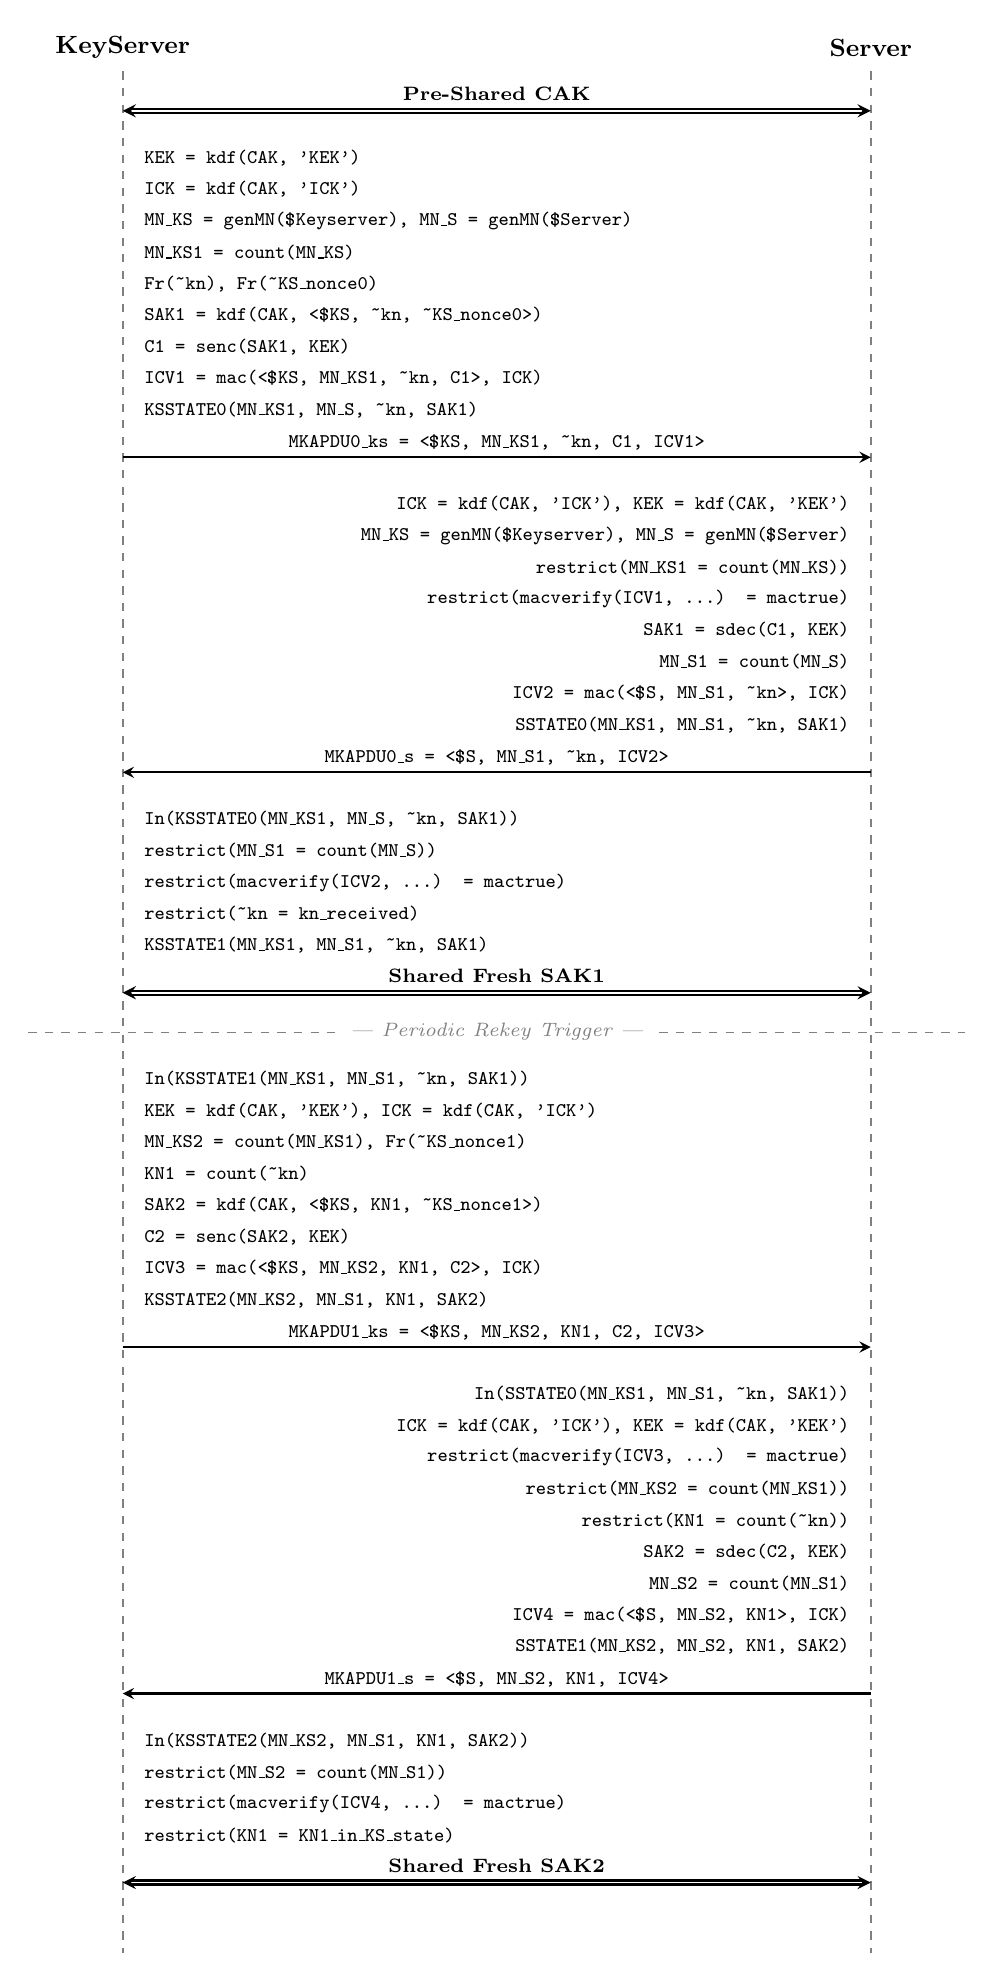
\begin{tikzpicture}[
  every node/.style={font=\scriptsize},
  arr/.style={->, >=stealth, thick},
  doublearr/.style={<->, >=stealth, thick, double},
  lbl/.style={font=\scriptsize\ttfamily, align=left},
  rlbl/.style={font=\scriptsize\ttfamily, align=right},
  msg/.style={font=\scriptsize\ttfamily, fill=white, inner sep=2pt}
]

% Lifelines
\def\KSx{0}
\def\Sx{9.5}

\node[font=\bfseries\small] (KS) at (\KSx, 0) {KeyServer};
\node[font=\bfseries\small] (S) at (\Sx, 0) {Server};

\draw[gray, dashed, thick] (\KSx, -0.3) -- (\KSx, -24.2);
\draw[gray, dashed, thick] (\Sx, -0.3) -- (\Sx, -24.2);

% Pre-shared CAK
\draw[doublearr] (\KSx, -0.8) -- node[above, font=\bfseries\scriptsize]{Pre-Shared CAK} (\Sx, -0.8);

% Initial - KeyServer Local
\node[lbl, anchor=west] at (\KSx+0.15, -1.4) {KEK = kdf(CAK, 'KEK')};
\node[lbl, anchor=west] at (\KSx+0.15, -1.8) {ICK = kdf(CAK, 'ICK')};
\node[lbl, anchor=west] at (\KSx+0.15, -2.2) {MN\_KS = genMN(\$Keyserver), MN\_S = genMN(\$Server)};
\node[lbl, anchor=west] at (\KSx+0.15, -2.6) {MN\_KS1 = count(MN\_KS)};
\node[lbl, anchor=west] at (\KSx+0.15, -3.0) {Fr(\textasciitilde kn), Fr(\textasciitilde KS\_nonce0)};
\node[lbl, anchor=west] at (\KSx+0.15, -3.4) {SAK1 = kdf(CAK, <\$KS, \textasciitilde kn, \textasciitilde KS\_nonce0>)};
\node[lbl, anchor=west] at (\KSx+0.15, -3.8) {C1 = senc(SAK1, KEK)};
\node[lbl, anchor=west] at (\KSx+0.15, -4.2) {ICV1 = mac(<\$KS, MN\_KS1, \textasciitilde kn, C1>, ICK)};
\node[lbl, anchor=west] at (\KSx+0.15, -4.6) {KSSTATE0(MN\_KS1, MN\_S, \textasciitilde kn, SAK1)};

% Msg 1
\draw[arr] (\KSx, -5.2) -- node[above, msg]{MKAPDU0\_ks = <\$KS, MN\_KS1, \textasciitilde kn, C1, ICV1>} (\Sx, -5.2);

% Initial - Server Local
\node[rlbl, anchor=east] at (\Sx-0.15, -5.8) {ICK = kdf(CAK, 'ICK'), KEK = kdf(CAK, 'KEK')};
\node[rlbl, anchor=east] at (\Sx-0.15, -6.2) {MN\_KS = genMN(\$Keyserver), MN\_S = genMN(\$Server)};
\node[rlbl, anchor=east] at (\Sx-0.15, -6.6) {restrict(MN\_KS1 = count(MN\_KS))};
\node[rlbl, anchor=east] at (\Sx-0.15, -7.0) {restrict(macverify(ICV1, \ldots) = mactrue)};
\node[rlbl, anchor=east] at (\Sx-0.15, -7.4) {SAK1 = sdec(C1, KEK)};
\node[rlbl, anchor=east] at (\Sx-0.15, -7.8) {MN\_S1 = count(MN\_S)};
\node[rlbl, anchor=east] at (\Sx-0.15, -8.2) {ICV2 = mac(<\$S, MN\_S1, \textasciitilde kn>, ICK)};
\node[rlbl, anchor=east] at (\Sx-0.15, -8.6) {SSTATE0(MN\_KS1, MN\_S1, \textasciitilde kn, SAK1)};

% Msg 2
\draw[arr] (\Sx, -9.2) -- node[above, msg]{MKAPDU0\_s = <\$S, MN\_S1, \textasciitilde kn, ICV2>} (\KSx, -9.2);

% Initial - KeyServer Confirm
\node[lbl, anchor=west] at (\KSx+0.15, -9.8) {In(KSSTATE0(MN\_KS1, MN\_S, \textasciitilde kn, SAK1))};
\node[lbl, anchor=west] at (\KSx+0.15, -10.2) {restrict(MN\_S1 = count(MN\_S))};
\node[lbl, anchor=west] at (\KSx+0.15, -10.6) {restrict(macverify(ICV2, \ldots) = mactrue)};
\node[lbl, anchor=west] at (\KSx+0.15, -11.0) {restrict(\textasciitilde kn = kn\_received)};
\node[lbl, anchor=west] at (\KSx+0.15, -11.4) {KSSTATE1(MN\_KS1, MN\_S1, \textasciitilde kn, SAK1)};

% Shared SAK1
\draw[doublearr] (\KSx, -12.0) -- node[above, font=\bfseries\scriptsize]{Shared Fresh SAK1} (\Sx, -12.0);

% Separator
\draw[dashed, gray] (-1.2, -12.5) -- (10.7, -12.5) node[midway, fill=white, font=\itshape\scriptsize]{--- Periodic Rekey Trigger ---};

% Rekey - KeyServer Local
\node[lbl, anchor=west] at (\KSx+0.15, -13.1) {In(KSSTATE1(MN\_KS1, MN\_S1, \textasciitilde kn, SAK1))};
\node[lbl, anchor=west] at (\KSx+0.15, -13.5) {KEK = kdf(CAK, 'KEK'), ICK = kdf(CAK, 'ICK')};
\node[lbl, anchor=west] at (\KSx+0.15, -13.9) {MN\_KS2 = count(MN\_KS1), Fr(\textasciitilde KS\_nonce1)};
\node[lbl, anchor=west] at (\KSx+0.15, -14.3) {KN1 = count(\textasciitilde kn)};
\node[lbl, anchor=west] at (\KSx+0.15, -14.7) {SAK2 = kdf(CAK, <\$KS, KN1, \textasciitilde KS\_nonce1>)};
\node[lbl, anchor=west] at (\KSx+0.15, -15.1) {C2 = senc(SAK2, KEK)};
\node[lbl, anchor=west] at (\KSx+0.15, -15.5) {ICV3 = mac(<\$KS, MN\_KS2, KN1, C2>, ICK)};
\node[lbl, anchor=west] at (\KSx+0.15, -15.9) {KSSTATE2(MN\_KS2, MN\_S1, KN1, SAK2)};

% Msg 3
\draw[arr] (\KSx, -16.5) -- node[above, msg]{MKAPDU1\_ks = <\$KS, MN\_KS2, KN1, C2, ICV3>} (\Sx, -16.5);

% Rekey - Server Local
\node[rlbl, anchor=east] at (\Sx-0.15, -17.1) {In(SSTATE0(MN\_KS1, MN\_S1, \textasciitilde kn, SAK1))};
\node[rlbl, anchor=east] at (\Sx-0.15, -17.5) {ICK = kdf(CAK, 'ICK'), KEK = kdf(CAK, 'KEK')};
\node[rlbl, anchor=east] at (\Sx-0.15, -17.9) {restrict(macverify(ICV3, \ldots) = mactrue)};
\node[rlbl, anchor=east] at (\Sx-0.15, -18.3) {restrict(MN\_KS2 = count(MN\_KS1))};
\node[rlbl, anchor=east] at (\Sx-0.15, -18.7) {restrict(KN1 = count(\textasciitilde kn))};
\node[rlbl, anchor=east] at (\Sx-0.15, -19.1) {SAK2 = sdec(C2, KEK)};
\node[rlbl, anchor=east] at (\Sx-0.15, -19.5) {MN\_S2 = count(MN\_S1)};
\node[rlbl, anchor=east] at (\Sx-0.15, -19.9) {ICV4 = mac(<\$S, MN\_S2, KN1>, ICK)};
\node[rlbl, anchor=east] at (\Sx-0.15, -20.3) {SSTATE1(MN\_KS2, MN\_S2, KN1, SAK2)};

% Msg 4
\draw[arr] (\Sx, -20.9) -- node[above, msg]{MKAPDU1\_s = <\$S, MN\_S2, KN1, ICV4>} (\KSx, -20.9);

% Rekey - KeyServer Confirm
\node[lbl, anchor=west] at (\KSx+0.15, -21.5) {In(KSSTATE2(MN\_KS2, MN\_S1, KN1, SAK2))};
\node[lbl, anchor=west] at (\KSx+0.15, -21.9) {restrict(MN\_S2 = count(MN\_S1))};
\node[lbl, anchor=west] at (\KSx+0.15, -22.3) {restrict(macverify(ICV4, \ldots) = mactrue)};
\node[lbl, anchor=west] at (\KSx+0.15, -22.7) {restrict(KN1 = KN1\_in\_KS\_state)};

% Shared SAK2
\draw[doublearr] (\KSx, -23.3) -- node[above, font=\bfseries\scriptsize]{Shared Fresh SAK2} (\Sx, -23.3);

\end{tikzpicture}%
}
\caption{Simplified two-party MKA protocol flow (initial session and rekey round) as specified in \texttt{MKA\_v10.spthy}. \$KS = KeyServer identity, \$S = Server identity, MN = Message Number counter, KN = Key Number counter.}
\label{fig:mka_flow}
\end{figure}

In the model, the \emph{Message Number} (MN) is a per-participant, monotonically increasing counter produced by \texttt{genMN} and advanced via \texttt{count}: $\mathit{MN\_KS1} = \mathtt{count}(\mathit{MN\_KS})$, $\mathit{MN\_KS2} = \mathtt{count}(\mathit{MN\_KS1})$, and analogously for the Server side. MNs protect against MKAPDU replay. The \emph{Key Number} (KN) identifies each key-generation epoch and advances at each rekey: $\mathit{KN1} = \mathtt{count}(\tilde{kn})$, where $\tilde{kn}$ is the fresh KN from the initial session. The state facts \texttt{KSSTATE0/1/2} and \texttt{SSTATE0/1} encode the protocol state machine and enforce strict sequencing between the initial session and the rekey round.

\section{Formal Analysis and Tamarin Prover}
\label{sec:analysis}

The Tamarin Prover~\cite{meier2013tamarin,basin2015tamarin} is a widely used tool for the automated symbolic verification of security protocols. It operates in the Dolev--Yao adversary model~\cite{dolevyao1983}: the adversary controls the network (can intercept, replay, modify, and inject messages) but cannot break cryptographic primitives (for example, cannot invert a hash, decrypt without the key, or forge a MAC).

\paragraph{Modelling language.} Tamarin protocols are specified as \emph{multiset rewriting rules} over a set of \emph{facts}. Each rule has the form
\[
  [\text{premise facts}] \xrightarrow{[\text{action facts}]} [\text{conclusion facts}]
\]
The premise specifies what facts must be present in the current system state, action facts annotate the rule firing with observable events, and the conclusion specifies what facts are produced. The special facts \texttt{Fr(x)} generate fresh nonces, \texttt{In(m)} receives a network message, and \texttt{Out(m)} sends one. Persistent facts (prefixed with \texttt{!}) survive consumption.

\paragraph{Equational theories.} Tamarin supports equational theories that model algebraic properties of cryptographic operations. For instance, \texttt{sdec(senc(m,k),k) = m} captures symmetric encryption/decryption, and \texttt{macverify(mac(M,K),M,K) = mactrue} captures MAC verification. The tool reasons about an arbitrary Dolev-Yao adversary that can apply these equations to derive new messages.

\paragraph{Restrictions and lemmas.} Restrictions (formerly called axioms) constrain the set of valid execution traces, allowing the modeller to express protocol-specific validity conditions (e.g., ``a MAC must verify''). Lemmas specify security properties in a fragment of first-order logic with time annotations:
\begin{itemize}
  \item \texttt{all-traces} lemmas express universal properties (safety, authentication, secrecy).
  \item \texttt{exists-trace} lemmas assert executability or demonstrate attack traces.
\end{itemize}
Tamarin employs a constraint-solving procedure with manual or automatic heuristics to discharge lemmas. Its soundness and completeness guarantees hold relative to the modelled equational theory.

\paragraph{Rule syntax and a concrete MKA example.} A Tamarin rule is declared as follows:
\begin{verbatim}
rule Setup_CAK:
  [ Fr(~cak) ]
  --[ CAKSetup(~cak) ]->
  [ !SharedCAK(~cak) ]
\end{verbatim}
The left-hand side (before \texttt{->}) lists premise facts; the right-hand side lists conclusion facts. For the MKA protocol, the initial session is captured by rules such as \texttt{Initial\_KeyServer\_Send}, \texttt{Initial\_Server\_Receive}, and \texttt{Initial\_KeyServer\_Confirm}, each encoding the state transitions depicted in Figure~\ref{fig:mka_flow}.

\paragraph{Monotonic counters and the \texttt{natural-numbers} builtin.} In our model, counters (MN and KN) are incremented using the \texttt{count(x)} function. To ensure sound reasoning about monotonicity, the \texttt{natural-numbers} builtin must be declared in the header of the \texttt{.spthy} file:
\begin{verbatim}
theory MKA_v10:
  builtins: natural-numbers

begin
...
end
\end{verbatim}
Without this builtin, Tamarin treats \texttt{count} as a generic function and may allow non-intuitive behaviour such as \texttt{count(x) = x} or \texttt{count(x) < x}, potentially invalidating proofs about session ordering.

\paragraph{Debugging and reproducibility.} When a lemma fails, Tamarin produces a concrete counterexample trace. This trace can be exported to LaTeX via the \texttt{--trace} option, which generates a \texttt{trace.tex} file that can be directly included in the paper. For reproducibility, all proof outputs—including \texttt{summary.pdf}, \texttt{trace.tex}, and the exact command-line invocation—are archived alongside the model in the repository.

\section{Our Formal Model}
\label{sec:model}

\subsection{Cryptographic Primitives and Equational Theory}

Our Tamarin model is built on the following builtins and functions:
\begin{itemize}
  \item \textbf{Symmetric encryption/decryption:} \texttt{senc}/\texttt{sdec} satisfying \texttt{sdec(senc(m,k),k) = m}.
  \item \textbf{Key derivation:} \texttt{kdf(key,label)} is modelled as an uninterpreted two-argument function; no algebraic identities are assumed, which captures the idealised one-way property of a KDF.
  \item \textbf{Message authentication:} \texttt{mac(M,K)} and \texttt{macverify(mac(M,K),M,K) = mactrue}; the equation ensures that the adversary can only produce a valid ICV if it knows the ICK.
  \item \textbf{Monotone counters:} \texttt{count(x)} models counter advancement and is used for both MN and KN progression. The \texttt{natural-numbers} builtin is enabled to provide a sound treatment of this function.
  \item \textbf{Message-number generation:} \texttt{genMN(\$Party)} is an uninterpreted function that assigns a fresh initial MN to a named party, ensuring per-party counter initialisation.
\end{itemize}

\subsection{Protocol Participants and Long-Term State}

\paragraph{CAK setup.} The rule \texttt{Setup\_CAK} generates a fresh CAK $\tilde{\mathit{cak}}$ and stores it as a persistent shared fact \texttt{!SharedCAK(\textasciitilde cak)}, available to both parties.

\paragraph{Derived keys.} Both participants independently compute
\[
  \mathit{kek} = \mathtt{kdf}(\mathit{cak}, \texttt{'KEK'}),\quad
  \mathit{ick} = \mathtt{kdf}(\mathit{cak}, \texttt{'ICK'})
\]
at the beginning of each protocol step, since both parties share the same CAK.

\subsection{Initial Session Rules}

\paragraph{Initial\_KeyServer\_Send.} The Key Server:
\begin{enumerate}
  \item Retrieves \texttt{!SharedCAK(\textasciitilde cak)}.
  \item Generates a fresh Key Number $\tilde{\mathit{kn}}$ and a fresh nonce $\widetilde{\mathit{KS\_nonce0}}$.
  \item Derives $\mathit{sak1} = \mathtt{kdf}(\mathit{cak}, \langle \$\mathit{Keyserver}, \tilde{\mathit{kn}}, \widetilde{\mathit{KS\_nonce0}}\rangle)$.
  \item Computes $\mathit{c1} = \mathtt{senc}(\mathit{sak1}, \mathit{kek})$.
  \item Computes $\mathit{icv1} = \mathtt{mac}(\langle \$\mathit{Keyserver}, \mathit{mn\_ks1}, \tilde{\mathit{kn}}, \mathit{c1}\rangle, \mathit{ick})$.
  \item Sends $\langle \$\mathit{Keyserver}, \mathit{mn\_ks1}, \tilde{\mathit{kn}}, \mathit{c1}, \mathit{icv1}\rangle$ and stores \texttt{KSSTATE0}.
\end{enumerate}
The action fact \texttt{SentInitialSAK} is recorded for use in the authentication lemmas.

\paragraph{Initial\_Server\_Receive.} The Server:
\begin{enumerate}
  \item Receives the MKAPDU from the network.
  \item Retrieves \texttt{!SharedCAK(\textasciitilde cak)} and verifies $\mathit{icv1}$ using a \texttt{\_restrict} action: \texttt{macverify(icv1, \ldots, ick) = mactrue}.
  \item Restricts the received MN to match the expected counter: $\mathit{mn\_ks1} = \mathtt{count}(\mathit{mn\_ks})$.
  \item Decrypts the payload: $\mathit{sak1} = \mathtt{sdec}(\mathit{c1}, \mathit{kek})$.
  \item Computes and sends its acknowledgement ICV2.
  \item Records \texttt{ServerAcceptedSAK} and stores \texttt{SSTATE0}.
\end{enumerate}

\paragraph{Initial\_KeyServer\_Confirm.} The Key Server receives the Server's ACK, verifies ICV2, checks that the received MN matches the expected counter, and transitions to \texttt{KSSTATE1}, recording \texttt{InitialSessionCompleted}.

\subsection{Rekey Rules}

The rekey phase mirrors the initial phase structurally, but it reads the previous state (\texttt{KSSTATE1}/\texttt{SSTATE0}) to enforce monotonicity. Specifically:

\begin{itemize}
  \item $\mathit{mn\_ks2} = \mathtt{count}(\mathit{mn\_ks1})$ and $\mathit{kn1} = \mathtt{count}(\tilde{\mathit{kn}})$ ensure both counters advance.
  \item A fresh nonce $\widetilde{\mathit{KS\_nonce1}}$ ensures SAK2 is independent of SAK1 even for identical KN paths.
  \item \texttt{Rekey\_KeyServer\_Send} records \texttt{RekeyStarted}, \texttt{Rekey\_Server\_Receive} records \texttt{RekeyAckPrepared}, and \texttt{Rekey\_KeyServer\_Confirm} records \texttt{RekeySessionCompleted}.
\end{itemize}

\subsection{Adversary Model and Compromise Rules}

We model a standard Dolev--Yao adversary augmented with two compromise rules:
\begin{itemize}
  \item \texttt{Reveal\_SAK}: exposes an initial SAK from \texttt{KSSTATE0}; records \texttt{RevealSAK}.
  \item \texttt{Reveal\_CAK}: exposes the CAK from \texttt{!SharedCAK}; records \texttt{RevealCAK}.
\end{itemize}
These rules allow the formulation of conditional security properties, for example that secrecy holds unless the CAK is revealed, and they capture the forward-secrecy limitations inherent in a pure pre-shared-key protocol.

Additionally, the rule \texttt{Malicious\_KeyServer\_Send} models a Key Server that uses the CAK to construct a well-formed MKAPDU carrying an arbitrary fresh SAK ($\widetilde{\mathit{fakeSAK}}$) instead of a properly KDF-derived one. This rule is used to probe the protocol's acceptance mechanism.

\subsection{Security Properties}
\label{sec:properties}

We specify twelve security properties as Tamarin lemmas. Table~\ref{tab:lemmas} summarises them. The checked entries show that the protocol is executable and that the main agreement, authentication, secrecy, and ordering properties hold under the stated assumptions. The two existence lemmas are especially important: they confirm that the model admits a valid execution trace, while also exposing the structural acceptance weakness in which a malicious Key Server can inject a non-KDF-derived SAK that the Server accepts.

\begin{table}[t]
\centering
\caption{Security lemmas verified against the MKA model.}
\label{tab:lemmas}
\setlength{\tabcolsep}{3pt}
\begin{tabular}{@{}p{2.6cm}p{1.3cm}p{2.3cm}c@{}}
\toprule
\textbf{Lemma} & \textbf{Type} & \textbf{Property} & \textbf{Res.} \\
\midrule
\texttt{executable} & exists-trace & Executability & \cmark \\
\texttt{initial\_agreement} & all-traces & Initial agreement & \cmark \\
\texttt{rekey\_agreement} & all-traces & Rekey agreement & \cmark \\
\texttt{server\_authentication\_initial} & all-traces & Server aliveness & \cmark \\
\texttt{server\_authentication\_rekey} & all-traces & Rekey aliveness & \cmark \\
\texttt{initial\_sak\_secrecy\_no\_reveal} & all-traces & SAK1 secrecy & \cmark \\
\texttt{rekey\_sak\_secrecy\_no\_reveal} & all-traces & SAK2 secrecy & \cmark \\
\texttt{rekey\_cannot\_start\_before\_initial} & all-traces & Ordering & \cmark \\
\texttt{rekey\_after\_initial\_completion} & all-traces & Ordering & \cmark \\
\texttt{key\_update} & all-traces & SAK1 $\neq$ SAK2 & \cmark \\
\texttt{key\_number\_progress} & all-traces & KN monotonicity & \cmark \\
\texttt{fresh\_rekey\_key} & all-traces & Rekey freshness & \cmark \\
\texttt{server\_only\_accepts\_kdf\_keys} & exists-trace & KDF bypass & \cmark \\
\texttt{accepts\_non\_kdf\_sak} & exists-trace & Malicious SAK & \cmark \\
\bottomrule
\end{tabular}
\end{table}

\subsection{Protocol Executability}

\begin{definition}[Executability]
The model is \emph{executable} if there exists at least one complete trace in which both \texttt{InitialSessionCompleted} and \texttt{RekeySessionCompleted} are observed.
\end{definition}

This is expressed as an \texttt{exists-trace} lemma and serves as a sanity check that the model does not over-restrict execution through contradictory restrictions.

\subsection{Agreement Properties}

\begin{definition}[Initial Agreement]
For every trace in which \texttt{InitialSessionCompleted}$(mn_{ks1}, mn_{s1}, kn, sak1)$ is observed at time $i$, there exists a strictly earlier time $j < i$ at which \texttt{SentInitialSAK}$(mn_{ks1}, kn, sak1)$ was recorded.
\end{definition}

This property captures \emph{non-injective agreement} (aliveness plus agreement on key material) from the Key Server's perspective: the Key Server cannot complete a session with a SAK it never sent.

\begin{definition}[Rekey Agreement]
Analogously, for every \texttt{RekeySessionCompleted} event, there exists an earlier \texttt{RekeyStarted} event with matching parameters.
\end{definition}

\subsection{Server Authentication}

\begin{definition}[Server Authentication --- Initial]
If \texttt{InitialSessionCompleted} is observed and the CAK has not been revealed, then \texttt{InitialAckPrepared} must have been observed earlier by the Server.
\end{definition}

This formalizes the requirement that the Key Server cannot consider a session complete unless the Server has actually processed the MKAPDU and generated a valid MAC acknowledgement, that is, the Server is \emph{alive} and has participated in the exchange.

\subsection{SAK Secrecy}

\begin{definition}[Initial SAK Secrecy]
If \texttt{InitialSessionCompleted} is observed, the SAK itself has not been directly revealed (\texttt{RevealSAK}), and the CAK has not been revealed (\texttt{RevealCAK}), then the adversary does not know $sak1$ (i.e., $K(sak1)$ is not derivable).
\end{definition}

The conditional structure reflects the inherent trust assumptions of a pre-shared-key protocol: compromise of the CAK transitively compromises all derived keys.

\subsection{Session Ordering and Key Freshness}

The lemmas \texttt{rekey\_cannot\_start\_}\allowbreak\texttt{before\_initial\_}\allowbreak\texttt{completion} and \texttt{rekey\_after\_}\allowbreak\texttt{initial\_completion} together express that the rekey sub-protocol is strictly sequenced after a successfully completed initial session. The lemma \texttt{key\_update} asserts $sak1 \neq sak2$, \texttt{key\_number\_progress} asserts $kn1 = \mathtt{count}(kn)$, and \texttt{fresh\_rekey\_key} asserts $sak2$ was not present in any initial session --- together these capture the semantic freshness and progression guarantees of the rekey mechanism.

\subsection{Structural Weakness: KDF-Bypass Attack}

\begin{definition}[Malicious SAK Acceptance]
There exists a trace in which \texttt{MaliciousSAKSent}($sak$) is observed before \texttt{ServerAcceptedSAK}($sak$), and $sak$ was never output by \texttt{KDFGeneratedSAK}.
\end{definition}

This exists-trace lemma captures the scenario in which a Key Server holding the CAK injects a fresh but non-KDF-derived SAK into a well-formed MKAPDU. The Server, having no independent means of verifying whether the SAK was derived through the prescribed KDF path or was arbitrary, accepts it. This is a \emph{structural} property of the protocol rather than a cryptographic break.
